\documentclass[11pt, dvipsnames, handout]{beamer}
\newtoggle{full}
\settoggle{full}{true}

\newtoggle{covered}
\settoggle{covered}{false}

\newtoggle{presentable}
\settoggle{presentable}{false}

\newtoggle{dualscreen}
\settoggle{dualscreen}{false}

\usepackage{pgfplots}
%\pgfplotsset{compat = newest}

\usepackage{pgfpages}

\setbeamertemplate{note page}{\pagecolor{yellow!5}\vfill \insertnote \vfill}
\usepackage{collect}
\definecollection{notes}
\newcounter{notestaken}

\usepackage{xpatch}

\usepackage{ulem}

\usepackage[framemethod=tikz]{mdframed}

\usepackage{scalerel}
\usepackage{calc}

%\usepackage{enumitem}
\setlength\fboxsep{.2em}

\usepackage{graphicx} % Allows including images
\usepackage{booktabs} % Allows the use of \toprule, \midrule and \bottomrule in tables

\xpatchcmd{\itemize}
  {\def\makelabel}
  {\setlength{\itemsep}{0.65 em}\def\makelabel}
  {}
  {}


\xpatchcmd{\beamer@enum@}
  {\def\makelabel}
  {\setlength{\itemsep}{0.65 em}\def\makelabel}
  {}
  {}


%\makeatletter
%\renewcommand{\itemize}[1][]{%
%  \beamer@ifempty{#1}{}{\def\beamer@defaultospec{#1}}%
%  \ifnum \@itemdepth >2\relax\@toodeep\else
%    \advance\@itemdepth\@ne
%    \beamer@computepref\@itemdepth% sets \beameritemnestingprefix
%    \usebeamerfont{itemize/enumerate \beameritemnestingprefix body}%
%    \usebeamercolor[fg]{itemize/enumerate \beameritemnestingprefix body}%
%    \usebeamertemplate{itemize/enumerate \beameritemnestingprefix body begin}%
%    \list
%      {\usebeamertemplate{itemize \beameritemnestingprefix item}}
%      {%
%        \setlength\topsep{1em}%NEW
%        \setlength\partopsep{1em}%NEW
%        \setlength\itemsep{1em}%NEW
%        \def\makelabel##1{%
%          {%
%            \hss\llap{{%
%                \usebeamerfont*{itemize \beameritemnestingprefix item}%
%                \usebeamercolor[fg]{itemize \beameritemnestingprefix item}##1}}%
%          }%
%        }%
%      }
%  \fi%
%  \beamer@cramped%
%  \raggedright%
%  \beamer@firstlineitemizeunskip%
%}
%
%
%
%
%
%\makeatother

%\setlist[beamer@enum@]{topsep=1 em}
%\let\origcheckmark\checkmark %screw you dingbat
%\let\checkmark\undefined %screw you dingbat
%\usepackage{dingbat} 
%\let\checkmark\origcheckmark %screw you dingbat






%\usepackage{fontawesome}

\usepackage{mathtools}
\usepackage{etoolbox, calculator}

\usepackage{xcolor}
\usepackage{tikz}
\usetikzlibrary{arrows.meta}
\usetikzlibrary{calc}
\usepackage[nomessages]{fp}
\usepackage{transparent}
\usepackage{accsupp}
%\usepackage{color, xcolor}

%colorblind-friendly palette
%\definecolor{dblue}{RGB}{51,34,136}
\definecolor{lblue}{RGB}{136,204,238}
%\definecolor{green}{RGB}{17,119,51}
\definecolor{tan}{RGB}{221,204,119}
%\definecolor{mauve}{RGB}{204,102,119}

\usepackage{tcolorbox}



\usepackage{xifthen}
\usepackage{nicefrac}
\usepackage{amsmath}
\usepackage{amsthm}
\usepackage{amssymb}
\theoremstyle{definition}
\newtheorem*{define}{Definition}
\newtheorem*{recall}{Recall}


\DeclareMathOperator{\tr}{tr}

\usepackage{multicol}
%\setlength{\columnsep}{1cm}

\usepackage{tablists, amsmath,vwcol, cancel, polynom}
\usetikzlibrary{shapes, patterns, decorations.shapes}
%\usepackage{tikzpeople}
\tikzstyle{vertex}=[shape=circle, minimum size=2mm, inner sep=0, fill]
\tikzstyle{opendot}=[shape=circle, minimum size=2mm, inner sep=0, fill=white, draw]

% common math quick commands
\newcommand{\nicedd}[2]{\nicefrac{\text{d}#1}{\text{d}#2}}
\newcommand{\dd}[2]{\dfrac{\text{d}#1}{\text{d}#2}}
\newcommand{\pd}[2]{\dfrac{\partial #1}{\partial#2}}
\renewcommand{\d}[1]{\text{d}#1}
\newcommand{\ddn}[3]{\dfrac{\text{d}^{#3}#1}{\text{d}#2^{#3}}}
\newcommand{\pdn}[3]{\dfrac{\partial^{#3}#1}{\partial#2^{#3}}}
\newcommand{\p}[0]{^{\prime}}
\newcommand{\pp}[0]{^{\prime\prime}}
\newcommand{\op}[2][\text{L}]{#1 \left[ #2 \right]}

\newcommand{\lap}[1]{\mathcal{L}\left\{#1\right\}}
\newcommand{\lapinv}[1]{\mathcal{L}^{-1}\left\{#1\right\}}
\newcommand{\lapint}[1]{\int_0^\infty e^{-st}#1dt}
\newcommand{\evalat}[2]{\Big|_{#1}^{#2}}

\newcommand{\paren}[1]{ \left( #1 \right)}

\newcommand{\haxis}[4][\normcolor]{\draw[#1, <->] (-#2,0)--(#3,0) node[right]{$#4$}; }


\newcommand{\axis}[4]{\draw[\normcolor, <->] (-#1,0)--(#2,0) 
node[right]{$x$};
\draw[help lines, <->] (0,-#3)--(0,#4) node[above]{$y$};}

\newcommand{\laxis}[6]{\draw[<->] (-#1,0)--(#2,0) 
node[right]{$#5$};
\draw[ <->] (0,-#3)--(0,#4) node[above]{$#6$};}
\newcommand{\xcoord}[2]{
	\draw (#1,.2)--(#1,-.2) node[below]{$#2$};}
\newcommand{\textnode}[3]{
	\draw (#1,#2) node[below]{$#3$};}
	
\newcommand{\nxcoord}[2]{
	\draw (#1,-.2)--(#1,.2) node[above]{$#2$};}
\newcommand{\ycoord}[2]{
	\draw (.2,#1)--(-.2,#1) node[left]{$#2$};}
\newcommand{\nycoord}[2]{
	\draw (-.2,#1)--(.2,#1) node[right]{$#2$};}
\newcommand{\dlim}{\displaystyle\lim}
\newcommand{\dlimx}[1]{\displaystyle\lim_{x \rightarrow #1}}
\newcommand{\stickfig}[2]{
	\draw (#1,#2) arc(-90:270:2mm);
	\draw (#1,#2)--(#1,#2-.5) (#1-.25,#2-.75)--(#1,#2-.5)--(#1+.25,#2-.75) (#1-.2,#2-.2)--(#1+.2,#2-.2);}	

%\newcounter{example}
%\setcounter{example}{1}
%\newcounter{preFrameExample}
%\AtBeginEnvironment{frame}{\setcounter{preFrameExample}{\value{example}}}
%\newcommand{\ex}[1]{
%	 \setcounter{example}{\value{preFrameExample}}
%	 \textcolor{green}{\small\fbox{Example \arabic{example}: #1}}\\[8pt]
%	\stepcounter{example}}
%\newcommand{\exans}[1]{
%	\SUBTRACT{\value{preFrameExample}}{1}{\n}
%	 \textcolor{green}{\small\fbox{Solution \n: #1}}\\[8pt]}
\mode<presentation> {

% The Beamer class comes with a number of default slide themes
% which change the colors and layouts of slides. Below this is a list
% of all the themes, uncomment each in turn to see what they look like.


\usetheme{CambridgeUS}
\usecolortheme[named=black]{structure}


\newcommand{\studentcolor}[0]{ForestGreen}
\newcommand{\normcolor}[0]{NavyBlue}
\newcommand{\alertcolor}{Red}

\setbeamercolor{normal text}{fg=\normcolor}
\setbeamercolor{frametitle}{fg=\normcolor}
\setbeamercolor{section in head/foot}{fg=Black, bg=Gray!20}
\setbeamercolor{subsection in head/foot}{fg=Green!70!Black, bg=Gray!10}
\setbeamercolor{alerted text}{fg=\alertcolor}
\setbeamerfont{alerted text}{series=\bf}
\setbeamertemplate{enumerate items}[default]
\setbeamercolor{enumerate item}{fg=\normcolor}

\setbeamertemplate{footline} % To remove the footer line in all slides uncomment this line
%\setbeamertemplate{footline}[page number] % To replace the footer line in all slides with a simple slide count uncomment this line

\setbeamertemplate{navigation symbols}{} % To remove the navigation symbols from the bottom of all slides uncomment this line
}

\newcommand{\alertbox}[1]{\tcbox[on line, colframe=\alertcolor, colback=White, left=2pt,right=2pt,top=2pt,bottom=2pt]{\usebeamercolor*{normal text}#1}}


\newcommand{\startstu}{\setbeamercolor{normal text}{fg=\studentcolor}\usebeamercolor*{normal text}\setbeamercolor{enumerate item}{fg=\studentcolor}\usebeamercolor*{enumerate item}}
\newcommand{\stopstu}{\setbeamercolor{normal text}{fg=\normcolor}\usebeamercolor*{normal text}\setbeamercolor{enumerate item}{fg=\normcolor}\usebeamercolor*{enumerate item}}

\newcommand{\takenote}[1]{ \begin{collect}{notes}{}{}{}{}  #1  \end{collect}  \addtocounter{notestaken}{1}} %\ifthenelse{\value{notestaken}>0}{\hrulefill\\}{}

\makeatletter
\newcommand{\cover}{\alt{\beamer@makecovered}{\beamer@fakeinvisible}}
\newcommand{\ucover}[1]{\iftoggle{full}{}{\beamer@endcovered}\stopstu#1\startstu\iftoggle{full}{}{\beamer@startcovered}}
\makeatother

\newcommand{\skippause}{ \addtocounter{beamerpauses}{-1}}
\newcommand{\blockpres}{ \skippause \pause }

\newcommand{\studentify}[1]{\startstu #1  \stopstu }
\newcommand{\student}[1]{\iftoggle{full}{ \pause  \studentify{#1} }{\iftoggle{covered}{\studentify{#1}}{\cover{  #1 }}}}
\newcommand{\cstudent}[1]{\student{\begin{center} #1 \end{center}}}
\newcommand{\fullonly}[1]{\iftoggle{full}{ #1}{}}
\newcommand{\presentonly}[1]{\iftoggle{presentable}{ #1}{}}

\usepackage{xparse}
\usepackage{xifthen}

% shortcuts for commonly-used presentation elements
%\NewDocumentCommand{\slide}{o m}
% {\IfValueTF{#1}{\begin{frame}[t]{#1}}{\begin{frame}[t]} #2 \end{frame}}

\newtoggle{iscovered}

\newcommand{\slide}[2][]{%
%\setcounter{notestaken}{0}
\takenote{#2} 
%\ifthenelse{\equal{#1}{}}{\begin{frame}[t]}{\begin{frame}[t]{#1}} #2 \ifthenelse{\value{notestaken}>0}{ \note{\includecollection{notes}}}{} \end{frame}%
\ifthenelse{\equal{#1}{}}{\begin{frame}[t]}{\begin{frame}[t]{#1}} #2 \iftoggle{covered}{\settoggle{iscovered}{true}}{\settoggle{iscovered}{false}}  \note{ \iftoggle{iscovered}{}{\settoggle{covered}{true}} #2 \iftoggle{iscovered}{}{\settoggle{covered}{false}} } \end{frame}%
%\setcounter{notestaken}{0}
}
\newcommand{\defn}[2][]{%
 \setcounter{listcounter}{0}%
\ifthenelse{\equal{#1}{}}{\begin{block}{Definition}}{\begin{block}{#1 :}}%
 #2 \vspace{0.25em} \ifthenelse{\value{listcounter}>0}{\skippause}{} \pause \end{block}%
}



\newcommand{\arr}[2]{\begin{array}{#1}#2\end{array}}
\newcommand{\mat}[2]{\left[\arr{#1}{#2}\right]}
\newcommand{\carray}[1]{\arr{c}{#1}}
\newcommand{\larray}[1]{\arr{l}{#1}}
\newcommand{\rarray}[1]{\arr{r}{#1}}
\newcommand{\colvec}[1]{\mat{c}{#1}}

\newcommand{\itmz}[1]{\addtocounter{listcounter}{1} \begin{itemize}#1 \end{itemize} }
\newcommand{\subitem}[1]{\addtocounter{listcounter}{1} \begin{itemize} \item #1 \end{itemize}}
%
\newcommand{\enum}[1]{\addtocounter{listcounter}{1} \begin{enumerate} #1  \end{enumerate}  }


\newcommand{\algnlbl}[1]{\begin{align}#1  \end{align}} 
\newcommand{\algn}[1]{\begin{align*}#1  \end{align*}} 
\newcommand{\lgn}[1]{ \action<+->{#1} }
\newcommand{\slgn}[1]{\iftoggle{full}{\action<+->{ \startstu #1 \stopstu}}{ \cover{ #1 } } \takenote{$#1$}}

\newcommand{\chckmrk}{\alert{\checkmark}}

\usepackage{pifont}
\newcommand{\xmark}{\alert{\text{\large \ding{55}}}}

\newcommand{\return}[0]{\raisebox{.5ex}{\rotatebox[origin=c]{180}{$\Lsh$}}}
\usepackage{pbox}
%\newcommand{\ex}[1]{\rotatebox[origin=c]{10}{\uline{ex}}:$\;$\pbox[t][][b]{0.9\linewidth}{#1}}
\newcommand{\ex}[1]{\uline{ex}:$\;$\pbox[t][][t]{0.9\linewidth}{#1}}
\newcommand{\eg}[1]{e.g.,$\;$\pbox[t][][t]{0.9\linewidth}{#1}}
\newcommand{\tikzplot}[8][]{%
\begin{tikzpicture}

\begin{scope}[]%
\clip(-#2,-#4) rectangle (#3,#5);%
#8%
\end{scope}%
\laxis{#2}{#3}{#4}{#5}{#6}{#7}%
#1
\end{tikzpicture}%
}


\newcommand{\cancelslide}[1]{%
\begingroup%
\setbeamertemplate{background canvas}{%
\begin{tikzpicture}[remember picture,overlay]%
\draw[line width=2pt,red!60!black] %
  (current page.north west) -- (current page.south east);%
\draw[line width=2pt,red!60!black] %
  (current page.south west) -- (current page.north east);%
\end{tikzpicture}}%
#1%
\endgroup%
}
\renewcommand{\CancelColor}{\color{red}}
\newcommand{\twocols}[3][0.5]{\begin{columns}\begin{column}{#1\textwidth}#2\end{column}\hspace{1em}\vrule{}\hspace{1em}\begin{column}{#1\textwidth}#3\end{column}\end{columns}}

\newcommand{\twomini}[5][1]{\calculatespace \begin{minipage}[t]{\columnwidth}\begin{minipage}[][#1\contentheight][t]{#2\columnwidth}#4\end{minipage}\hfill\begin{minipage}[][#1\contentheight][t]{#3\columnwidth}#5\end{minipage}\end{minipage}}

\newcommand{\threemini}[7][1]{\calculatespace \begin{minipage}[t]{\columnwidth}\begin{minipage}[][#1\contentheight][t]{#2\columnwidth}#5\end{minipage}\hfill\begin{minipage}[][#1\contentheight][t]{#4\columnwidth}#6\end{minipage}\hfill\begin{minipage}[][#1\contentheight][t]{#3\columnwidth}#7\end{minipage}\end{minipage}}


\newcounter{listcounter}
\setcounter{listcounter}{0}



\newif\ifsidebartheme
\sidebarthemetrue

\newdimen\contentheight
\newdimen\contentwidth
\newdimen\contentleft
\newdimen\contentbottom
\makeatletter
\newcommand*{\calculatespace}{%
\contentheight=\paperheight%
\ifx\beamer@frametitle\@empty%
    \setbox\@tempboxa=\box\voidb@x%
  \else%
    \setbox\@tempboxa=\vbox{%
      \vbox{}%
      {\parskip0pt\usebeamertemplate***{frametitle}}%
    }%
    \ifsidebartheme%
      \advance\contentheight by-1em%
    \fi%
  \fi%
\advance\contentheight by-\ht\@tempboxa%
\advance\contentheight by-\dp\@tempboxa%
\advance\contentheight by-\beamer@frametopskip%
\ifbeamer@plainframe%
\contentbottom=0pt%
\else%
\advance\contentheight by-\headheight%
\advance\contentheight by\headdp%
\advance\contentheight by-\footheight%
\advance\contentheight by4pt%
\contentbottom=\footheight%
\advance\contentbottom by-4pt%
\fi%
\contentwidth=\paperwidth%
\ifbeamer@plainframe%
\contentleft=0pt%
\else%
\advance\contentwidth by-\beamer@rightsidebar%
\advance\contentwidth by-\beamer@leftsidebar\relax%
\contentleft=\beamer@leftsidebar%
\fi%
}
\makeatother


\iftoggle{dualscreen}{\setbeameroption{show notes on second screen=right}}{}

\usepackage{gensymb}
\begin{document}

\slide[The Heat Equation and the Laplacian]{
Recall the 1D heat equation \[u_t=\alpha u_{xx} = \alpha \pdn{}{x}{2} u(x,t)\]\vfill
In higher dimentions ($x$, $y$, $\dots$) this becomes \student{ \algn{u_t &= \alpha\left( u_{xx} + u_{yy} + \dots \right) \\ &=\alpha \Delta u }
$\Delta$ is the Laplacian operator \[ \Delta =  \pdn{}{x}{2}  + \pdn{}{y}{2} + \dots  \quad  = \vec{\nabla} \cdot \vec{\nabla} \qquad \text{with } \vec{\nabla} = \mat{c}{ \pd{}{x} \\\\  \pd{}{y} \\\\ \vdots}   \]}
}

\slide[Steady State Heat Equation]{
If a steady state heat distribution is attained, we have $u_t\to0$.\vfill In 1D this gave us \[ 0 = u_{xx} \qquad \student{\Rightarrow u_\infty(x)=C_1x+C_2} \]
\vfill
\student{Given some boundary conditions, we can find $u_\infty$.}\vfill
\ex{Suppose our domain is $x\in[0,L]$ with $u(0,t)=a$ and $u(L,t)=b$}\vfill
\student{\[u_\infty(x) = a + \frac{b-a}{L}x\]}
}

\slide[Laplace's Equation]{
In higher dimensions, we need to solve Laplace's Equation \[ \Delta u = 0\]
\vfill
Restrciting ourselves to 2 dimensions, we get\[ u_{xx} + u_{yy} = 0\]
\vfill
No longer as simple as finding linear functions\vfill
\ex{$u(x,y)=x^2-y^2$}
\[u_{xx} =2, \qquad u_{yy}=-2 \qquad \Rightarrow u_{xx} + u_{yy} =0 \]
\vfill
Solutions to Laplace's Equation are called \alert{harmonic functions}
}
\slide[Boundary Conditions - Dirichlet Problem]{
Consider a region in the $x,y$-plane. \vfill We specify certain values of some unknown function $u(x,t)$ along the boundaries of the region. \vfill We then try to find a solution  to the Laplace equation \[ u_{xx} + u_{yy} = 0\] defined on this region such that  agrees with the values we specified on the boundary.
}

\slide[Boundary Conditions - Dirichlet Problem]{
\ex{Consider a rectangular region of width $w$ and height $h$.}

\vfill
Boundary values are zero at three of the four edges, and obey some arbitrary function $f(x)$ along the fourth edge.\vfill
\twomini[.4]{.5}{.5}{\algn{\Delta u &=0 \\
u(0,y)&=0 &\text{for } 0<y<h\\
u(x,h)&=0 &\text{for } 0<x<w\\
u(w,y)&=0 &\text{for } 0<y<h\\
u(x,0)&=f(x) &\text{for } 0<x<w }}{\vspace{.5cm} \centerline{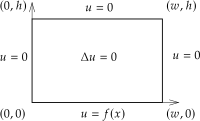
\includegraphics[width=.85\columnwidth]{images/dirichsetup.pdf}}}

}

\slide[Solving Dirichlet Problems]{
\[ u_{xx}+u_{yy} = 0 \]
Separation of Variables: \[u(x,y) = X(x)Y(y)\]
\student{\algn{X\pp Y+XY\pp &= 0 \\
\frac{X\pp(x)}{X(x)} = -\frac{Y\pp(y)}{Y(y)} &= -\lambda = \text{const.}}\vfill
\twomini[.15]{.5}{.5}{\[X\pp+\lambda X =0 \]}{\[Y\pp-\lambda Y =0 \]}

}
}

\slide[Solving Dirichlet Problems]{
\twomini[.35]{.5}{.45}{\[X\pp+\lambda X =0 \]}{ \centerline{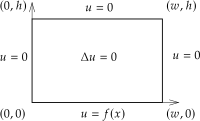
\includegraphics[width=.85\columnwidth]{images/dirichsetup.pdf}} }
\vfill
What are the boundary conditions? What are the allowed solution and values of $\lambda$?
\vfill
\student{
BCs: $X(0)=X(w)=0$

\[X_n(x)= \sin \left( \frac{n\pi}{w} x \right)  \qquad \lambda_n = \left(\frac{n\pi}{w}\right)^2\]
}
}

\slide[Solving Dirichlet Problems]{
\twomini[.35]{.5}{.45}{\[Y\pp-\lambda Y =0 \] \vfill\[ \lambda = \left(\frac{n\pi}{w}\right)^2\] \vfill }{ \centerline{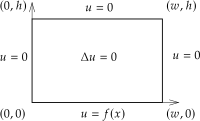
\includegraphics[width=.85\columnwidth]{images/dirichsetup.pdf}} }
\vfill
What are the boundary conditions? What types of solutions do we obtain?
\vfill
\student{
BCs: $Y(h)=0$, less clear what is going on for $y=0$.\\
Try $Y_n=e^{ry}$
\algn{r^2e^{ry} - \left(\frac{n\pi}{w}\right)^2 e^{ry}&=0 \\
r^2 = \left(\frac{n\pi}{w}\right)^2&=0& \Rightarrow r&=\pm\frac{n\pi}{w} }\[Y_n(y) = Ae^{\frac{n\pi}{w} y} + B e^{-\frac{n\pi}{w} y}\]
}
}

\slide[]{\vspace{-1em}\[Y_n(y) = Ae^{\frac{n\pi}{w} y} + B e^{-\frac{n\pi}{w} y} \qquad \text{with } Y(h)=0 \]\vspace{-2em}
\student{\algn{Y(h)=0&= Ae^{\frac{n\pi}{w} h} + B e^{-\frac{n\pi}{w} h} \qquad\quad \Rightarrow A= - Be^{-2 \frac{n\pi}{w} h }\\\\
Y_n(y) &= B \left[- e^{-2\frac{n\pi}{w}h} e^{\frac{n\pi}{w} y} + e^{-\frac{n\pi}{w}y} \right] \\
&=B\left[ - e^{-\frac{n\pi}{w}h} e^{\frac{n\pi}{w} (y-h)}  +  e^{-\frac{n\pi}{w}h} e^{-\frac{n\pi}{w} (y-h)} \right]\\\
&=\underbrace{B   e^{-\frac{n\pi}{w}h} }_{\text{arbitrary}} \underbrace{\left[   e^{-\frac{n\pi}{w} (y-h)} - e^{\frac{n\pi}{w} (y-h)}  \right]}_{\propto \sinh}\\
&=a_n \sinh \left( \frac{n\pi}{w} (h-y)\right)
}\vfill\[u_{n}(x,y) = a_n \sin \left( \frac{n\pi}{w}x \right) \sinh \left( \frac{n\pi}{w} (h-y)\right)\]\vfill
Eigensolution of the Laplacian that satifies the zero boundary conditions on the 3 sides.
}
}

\slide[The non-zero boundary condition]{\vspace{-2em}\[u_{n}(x,y) = a_n \sin \left( \frac{n\pi}{w} x \right) \sinh \left( \frac{n\pi}{w} (h-y)\right), \quad u(x,y)=\sum_{n=1}^{\infty} u_n(x,y)\]\vfill
$u(x,0)=f(x) $ - Express the boundary condition as Fourier Series\vfill
\student{
Given the appearance of our $u_n$, we clearly need a Sine series
\algn{f(x) &=\sum_{n=1}^{\infty} b_n \sin \left( \frac{n\pi}{w} x \right) \qquad \text{with } b_n=\frac{2}{w} \int_0^w f(x) \sin \left( \frac{n\pi}{w} x \right) dx  \\
u(x,0)&=f(x) = \sum_{n=1}^{\infty} a_n \sin \left( \frac{n\pi}{w} x \right) \sinh \left( \frac{n\pi}{w} h \right) \intertext{need equality between the two series}
\Rightarrow a_n &= \frac{b_n}{ \sinh \left( \frac{n\pi}{w} h \right) } 
}
}
}

\slide[The Hyperbolic Functions]{
\twomini[.92]{.5}{.5}{\algn{\sinh x &=\frac{e^x-e^{-x}}{2}\\ \cosh x &=\frac{e^x+e^{-x}}{2}\\ \tanh &=\frac{\cosh x}{\sinh x} =\frac{e^x+e^{-x}}{e^x-e^{-x}}  \\\\\\\
\dd{}{x}\sinh x &=\cosh x\\
\dd{}{x}\cosh x &=\sinh x\\
\dd{}{x}\tanh x &=1-\tanh^2 x = \frac{1}{\cosh^2 x}
}}{\includegraphics[width=\columnwidth]{images/Sinh_cosh_tanh.pdf}}


\hfill \tiny source: Wikipedia

}

\slide[Boundary conditions on two sides]{
\ex{Consider a rectangular region of width $1$ and height $1$.}
\vspace{-1em}
\algn{\Delta u &=0 \\
u(0,y)&=0 &\text{for } 0<y<h\\
u(x,h)&=0 &\text{for } 0<x<w\\
u(w,y)&=\sin(3\pi x) &\text{for } 0<y<h\\
u(x,0)&=x &\text{for } 0<x<w }
\vfill
 \centerline{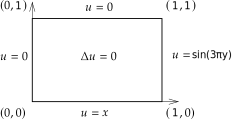
\includegraphics[width=.5\columnwidth]{images/dirichsetup2.pdf}}
\vfill

}

\slide[Breaking it down by directions]{
\twomini[.55]{.45}{.45}{ South Problem 
\vfill
\centerline{  \includegraphics[height=3cm]{images/dirichsetup2_south.pdf}}}{ East Problem
\vfill
 \centerline{\includegraphics[height=3cm]{images/dirichsetup2_east.pdf}}}

\vfill
\student{\[u(x,y)=u_N+u_S+u_E+u_W\]}
\vfill
The west and north problems have zero solutions, no need to solve them.

}


\slide[The South Problem]{
Special case of the previous problem we did with $f(x)=x$
\student{
\[u_s(x,y)=\sum_{n=1}^{\infty}  a_n \sin \left( n\pi x \right) \sinh \left( n\pi (1-y)\right)\]
\vfill
\algn{ a_n &= \frac{b_n}{\sinh(n\pi)} & b_n&=2 \int_0^1 x \sin(n \pi x)dx\\
&&&=-2\frac{(-1)^n}{n\pi}
}
}
\vfill
\tiny\url{https://www.wolframalpha.com/input?i=integral+of+x*sin\%28n*pi*x\%29+from+0+to+1+assuming+n+is+an+integer}
}

\slide[The East Problem]{
\twomini[.4]{.5}{.45}{\algn{\Delta u_E &=0 \\
u_E(0,y)&=0 &\text{for } 0<y<h\\
u_E(x,h)&=0 &\text{for } 0<x<w\\
u_E(w,y)&=\sin(3\pi y) &\text{for } 0<y<h\\
u_E(x,0)&=0 &\text{for } 0<x<w }}{\vspace{.5cm} \centerline{\includegraphics[width=.85\columnwidth]{images/dirichsetup2_east.pdf}}}
\vfill
\student{
\[X\pp+\lambda X =0 \qquad Y\pp-\lambda Y =0 \]
Now we have two zero BCs for $Y(y)$
\[Y(0)=Y(1)=0 \qquad \Rightarrow Y_n(y)=\sin (n\pi y)\]
with \[\lambda_n=-(n\pi)^2\]
}
}
\slide[The East Problem]{
\twomini[.4]{.5}{.45}{\[X\pp+\lambda X =0  \qquad \text{with } \lambda=-(n\pi)^2  \]}{\vspace{.5cm} \centerline{\includegraphics[width=.85\columnwidth]{images/dirichsetup2_east.pdf}}}
\student{
\algn{X\pp -(n\pi)^2 X &= 0\\
X(x) &= Ae^{n\pi x} +Be^{-n\pi x}\\
\text{BC @ x=0:} \qquad 0 &= A+B&B&=-A\\
X(x)& = A(e^{n\pi x} - e^{-n\pi x})\\
&=a_n \sinh (n \pi x) 
}
\[u_{n}(x,y) = a_n \sin \left( n\pi y \right) \sinh \left( n\pi x\right)\]
}
}

\slide[The East Problem]{
\twomini[.4]{.5}{.45}{\[u_{n}(x,y) = a_n \sin \left( n\pi y \right) \sinh \left( n\pi x\right)\]  \[u_E =\sum_{n=1}^\infty u_n(x,y) \]}{\vspace{.5cm} \centerline{\includegraphics[width=.85\columnwidth]{images/dirichsetup2_east.pdf}}}
\student{
BC @ x=1
\algn{u(1,y) &= \sin(3\pi y) = \sum_n a_n \sin(n \pi y) \sinh(n\pi)\\
a_n &= \begin{cases} \frac{1}{\sinh(3\pi)} & n=3 \\ 0 &\text{otherwise}  \end{cases}}\[u_E = u_3(x,y) = \frac{\sinh(3\pi x)}{\sinh(3\pi)}\sin(3\pi y)\]
}
}

\slide{\vfill
 \centerline{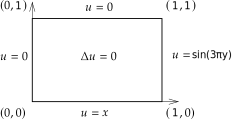
\includegraphics[width=.5\columnwidth]{images/dirichsetup2.pdf}}
\algn{u(x,t) &= u_S + u_E +\cancelto{0}{u_N} +\cancelto{0}{u_W}\\\\
&=\sum_{n=1}^{\infty}  -2\frac{(-1)^n}{n\pi} \sin \left( n\pi x \right) \sinh \left( n\pi (1-y)\right) \\& \phantom{=}+\frac{\sinh(3\pi x)}{\sinh(3\pi)}\sin(3\pi y)}
\vfill

}

\slide[Separation of Variables on Rectangular Domains]{
\itmz{\item General Approach: $u(x,y)=u_N+u_S+u_E+u_W$\vfill
\item Each $u_I$ solves a Dirichlet problem with \uline{one} non-zero BC
\subitem{If a problem has all zero BCs, then $u_I$ is zero}
\algn{ u_N &= \sum_n a_n \sin \left( \frac{n\pi}{w}x \right) \sinh \left( \frac{n\pi}{w} y\right)\\
u_S &= \sum_n b_n \sin \left( \frac{n\pi}{w}x \right) \sinh \left( \frac{n\pi}{w} (h-y)\right)\\
u_E &= \sum_n c_n \sin \left( \frac{n\pi}{h}y \right) \sinh \left( \frac{n\pi}{h} x\right)\\
u_W &= \sum_n d_n \sin \left( \frac{n\pi}{h} y \right) \sinh \left( \frac{n\pi}{h} (w-x)\right)
}\vfill
\item Find the arbitrary coefficients by comparing each series solution to a Fourier series of the non-zero BC.
}\vfill


}

\end{document}